\documentclass[
 reprint,
%superscriptaddress,
%groupedaddress,
%unsortedaddress,
%runinaddress,
%frontmatterverbose, 
%preprint,
%preprintnumbers,
%nofootinbib,
%nobibnotes,
%bibnotes,
 amsmath,amssymb,
 aps,
pra,
%prb,
%rmp,
%prstab,
%prstper,
floatfix,
]{revtex4-2}

\usepackage{graphicx}% Include figure files
\usepackage{dcolumn}% Align table columns on decimal point
\usepackage{bm}% bold math
%\usepackage{hyperref}% add hypertext capabilities
%\usepackage[mathlines]{lineno}% Enable numbering of text and display math
%\linenumbers\relax % Commence numbering lines

%\usepackage[showframe,%Uncomment any one of the following lines to test 
%%scale=0.7, marginratio={1:1, 2:3}, ignoreall,% default settings
%%text={7in,10in},centering,
%%margin=1.5in,
%%total={6.5in,8.75in}, top=1.2in, left=0.9in, includefoot,
%%height=10in,a5paper,hmargin={3cm,0.8in},
%]{geometry}

\begin{document}

\preprint{APS/123-QED}

\title{Quasienergy and Shaken Optical lattice}% Force line breaks with \\
%\thanks{A footnote to the article title}%

\author{XiaoHui, HU}
%  \altaffiliation[Also at ]{Physics Department, XYZ University.}%Lines break automatically or can be forced with \\
% \author{Second Author}%
%  \email{Second.Author@institution.edu}
% \affiliation{%
%  Authors' institution and/or address\\
%  This line break forced with \textbackslash\textbackslash
% }%

% \collaboration{MUSO Collaboration}%\noaffiliation

% \author{Charlie Author}
%  \homepage{http://www.Second.institution.edu/~Charlie.Author}
% \affiliation{
%  Second institution and/or address\\
%  This line break forced% with \\
% }%
% \affiliation{
%  Third institution, the second for Charlie Author
% }%
% \author{Delta Author}
% \affiliation{%
%  Authors' institution and/or address\\
%  This line break forced with \textbackslash\textbackslash
% }%

% \collaboration{CLEO Collaboration}%\noaffiliation

\date{\today}% It is always \today, today,
             %  but any date may be explicitly specified

% \begin{abstract}
% An article usually includes an abstract, a concise summary of the work
% covered at length in the main body of the article. 
% \begin{description}
% \item[Usage]
% Secondary publications and information retrieval purposes.
% \item[Structure]
% You may use the \texttt{description} environment to structure your abstract;
% use the optional argument of the \verb+\item+ command to give the category of each item. 
% \end{description}
% \end{abstract}

%\keywords{Suggested keywords}%Use showkeys class option if keyword
                              %display desired
\maketitle

%\tableofcontents

\section{\label{sec:level1}Introduction}

Optical lattice is a pure and highly controllable platform in quantum field.
It becomes more and more useful and one of the most platform to simulate quantum many-body system.%ref...
Optical lattice is a artificial periodic structure.
In this way the optical lattice can simulate the crystal structure in condensed matter physics. 
Moreover, the properties of cold atoms in the optical lattice are very similar to those of electrons in the solid lattice, 
so the cold atoms in the optical lattice can be used to simulate the complex crystal model.%ref...
The optical lattice system can be used to study the related problems of quantum phase transition. 
In 2002, Bloch et al. observed the superfluid Mott phase transition of boson in the Bose Einstein condensate of Rb in three-dimensional optical lattice.%ref
The cold atoms in the optical lattice are not easily disturbed by the outside world, it has great development potential in time measurement.%ref

Using time period to change the potential in the optical lattice, so the potential is both space period and time period.
We can get the shaken optical lattice. Floquet theory can be used in the shaken optical lattice.%ref...
Floquet theory is very important in quantum mechanics. It is widely used to study various physical phenomena, 
such as the Chaos Quantum ratchet, the electronic transition in the semiconductor heterostructure, and dynamic tunneling.%ref...
In this paper, we study the physical properties and modulation methods of the shaken optical lattice system after the introduction of time period.%ref...

\section{Shaken Optical Lattice}
The optical lattice is produced by a pair of laser beams as Fig.~\ref{fig1}.
\begin{figure}[b]
  \includegraphics[width = 6cm]{fig1.eps}
  \caption{\label{fig1} The optical lattice is produced by a pair of laser beams.The two laser beams propagating in the opposite direction form a standing wave field. 
  This force is periodic. The corresponding periodic optical potential well is obtained.}
\end{figure}
The potential function of one-dimensional optical lattice is as follows:
\begin{equation}
  V=\frac{V_{0}}{2} \cos (2 k x)
  \label{eq1}
\end{equation}
However, when the two lasers are not exactly the same (for example, there is a difference between the frequency or phase), 
the form of the potential function will change, and the standing wave field will also move, causing changes at the system level.
This is the shaken optical lattice.
Shaken optical lattice can also simulate quantum systems, but its advantage is time period term. 
Many novel physical phenomena can be induced and deduced by spatiotemporal periodic. 
This is reason we focus on shaken optical lattice.

The processing of two laser beams is also called modulation mode. The potential function of the potential well will also change accordingly:
\begin{equation}
  V=\frac{V_{0}}{2} \cos \left(2 k x+X_{0}(t)\right)
  \label{eq2}
\end{equation}

Now there will be time-dependent term in the potential function, which will affect the whole optical lattice system. 
Then the Hamiltonian of the system becomes:
\begin{equation}
  H=\frac{p^{2}}{2 M}+V_{l a t}(x, t)
  \label{eq3}
\end{equation}

$V_{l a t}(x, t)$ is not only a space period, but also related to time, for the convenience of later calculation. 
We need to simplify that. After simplification, we can get:%ref...
\begin{equation}
  H^{\prime}=\frac{\left[\widetilde{\boldsymbol{p}}+M \dot{X}_{0}\right]^{2}}{2 M}+V_{l a t}(x)-\frac{1}{2} M \dot{X}_{0}^{2}
  \label{eq4}
\end{equation}
There is a time-dependent vector potential in the shaken optical lattice from the above formula
\begin{equation}
  A=-M \dot{X}_{0}
  \label{eq5}
\end{equation}
This vector potential will get a force field.
\begin{equation}
  \mathbf{F}=\frac{\partial \mathbf{A}}{\partial \mathrm{t}}=-\mathrm{M} \ddot{X}_{0}
  \label{eq6}
\end{equation}

In the case of tight binding approximation of single particle model, 
the corresponding time-dependent Schrodinger equation is given by the so-called Houston State.
These states give the time-dependent quasi momentum relations as follows
\begin{equation}
  q(t)=-\frac{F_{0}}{\hbar \omega} \cos (\omega t)
  \label{eq7}
\end{equation}
According to the relation of the lowest energy level in the tight binding approximation, we can get
\begin{equation}
  E^{(0)}(q)=-2 J_{0} \cos (d q)
\end{equation}
We can get the equivalent energy band relation under tight binding approximation by taking the above relation into and taking the time average in a period.
\begin{equation}
  E_{e f f}(q)=\frac{1}{T} \int_{0}^{T} d t E^{(0)}(q(t))=-2 J_{e f f} \cos (d q)
\end{equation}
Where $J_{e f f}$ is the equivalent transition matrix element, 
which is obtained by rescaling the normal transition matrix element through the zero order Bessel function in the Fig.~\ref{fig2}
\begin{figure}[b]
  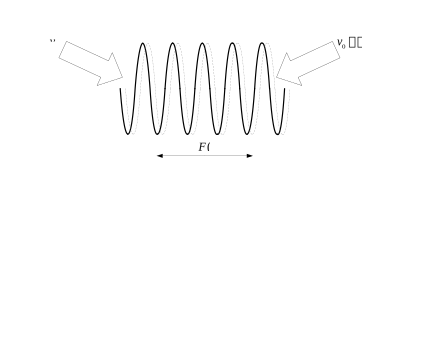
\includegraphics[width = 6cm]{fig2.eps}
  \caption{\label{fig2} Zero order Bessel function.The positions of zero points of Zero order Bessel function}
\end{figure}
\begin{equation}
  J_{e f f}=J_{0} \mathcal{J}_{0}\left(\frac{d F_{0}}{\hbar \omega}\right)=J_{0} \mathcal{J}_{0}\left(K_{0}\right)
\end{equation}
$K_{0}$ is a dimensionless parameter, which describes the intensity of modulation mode.

\section{The Modulation}

Different modulation methods will lead to different forms of potential functions, %ref...
which will affect the relationship between intensity $K_{0}$. 
The following describes the relationship between various vibration modes and strength $K_{0}$.
\begin{figure}[b]
  \includegraphics[width = 6cm]{fig3.eps}
  \caption{\label{fig3} Two modulation methods of shaken optical lattice.
  Schematic diagram of two different modulation modes, FIG. A is frequency modulation. 
  The frequency difference between the two laser beams results in the deviation of the optical potential well; 
  Figure B shows the phase modulation. The phase difference between laser beam and its reflected wave causes the vibration of optical lattice}
\end{figure}

\subsection{Frequency Modulation}
First, it is frequency modulation.%ref...
When the frequency difference between two lasers is $\Delta v=\Delta v_{\max } \sin (\omega t)$.
The actual potential field of the shaken optical lattice is
\begin{equation}
  V_{\text {lat }}=\frac{V_{0}}{2} \cos \left(2 k\left[x-\frac{\lambda \Delta v_{\max }}{2 \omega} \cos (\omega t)\right]\right)
  \label{eq11}
\end{equation}

From the Eqs.~\ref{eq11}, we can get the modulation intensity
\begin{equation}
  K_{0}=\frac{\mathrm{F}_{0} d}{\hbar \omega}=\frac{M d^{2} \omega \Delta v_{\max }}{\hbar \omega}=\frac{\pi^{2}}{2} \cdot \frac{\Delta v_{\max }}{\omega_{r e c}}
\end{equation}
where $\omega_{r e c}=\frac{E_{r e c}}{\hbar}$ is recoil frequency.
From the above formula, we can see the relationship between frequency modulation mode and modulation intensity. 
The modulation intensity $K_{0}$ is directly proportional to the amplitude of frequency modulation and inversely proportional to the recoil frequency. 
It is not related to the frequency of modulation. 

Of course, the recoil frequency is related to the selected cold atoms. Once selected, it will not change.
For example, $^{87} R b$ its recoil frequency is $3.24 k \times 2\pi Hz$. The relationship between modulation intensity and frequency modulation amplitude can be analyzed.
%As Fig.~\ref{fig5}.

% \begin{figure}[b]
%   \includegraphics[width = 6cm]{fig5.eps}
%   \caption{\label{fig5} The relationship between frequency modulation amplitude and modulation intensity}
% \end{figure}

\subsection{Phase Modulation}

Then, Modulation phase is another commonly used modulation method.%ref...
The system consists of a standing wave formed by the interference of the reflected light of a laser beam reflected by a plane mirror with the initial incident light. 
When the plane mirror is periodically shifted, it will change the phase of the reflected light, %ref...
so as to achieve the purpose of periodic movement of the optical lattice.

% \begin{figure}[b]
%   \includegraphics[width = 6cm]{fig4.eps}
%   \caption{\label{fig4} The phase modulation. The phase difference between laser beam and its reflected wave causes the vibration of optical lattice}
% \end{figure}

The displacement equation of plane mirror is set as $X(t)=\Delta x_{\max } \cos (\omega t)$, then the potential field in the optical lattice is
\begin{equation}
  V_{l a t}=\frac{V_{0}}{2} \cos \left(2 k\left[x-\Delta x_{\max } \cos (\omega t)\right]\right)
\end{equation}

In this modulation mode, the modulation intensity is
\begin{equation}
  K_{0}=\frac{\mathrm{F}_{0} d}{\hbar \omega}=\frac{M \omega^{2} \omega \Delta x_{\max } d}{\hbar \omega}=\frac{\pi^{2}}{2} \frac{\omega}{\omega_{r e c}} \frac{\Delta x_{\max }}{d}
\end{equation}
The modulation intensity is related to modulation frequency, modulation amplitude, recoil frequency and lattice constant. 
Similarly, the recoil frequency and lattice constant are related to the constructed shaken optical lattice system. 
In this way, we analyze the relationship between modulation intensity and modulation frequency.

% \subsection{Hybrid Modulation}

% \section{Dynamic Localization}

% \section{High-order Sideband generation}

% \section{Conclusion}


% \begin{figure}[b]
%   \includegraphics[width = 6cm]{fig6.eps}
%   \caption{\label{fig6} figure6}
% \end{figure}

% \begin{figure}[b]
%   \includegraphics[width = 6cm]{fig7.eps}
%   \caption{\label{fig7} figure7}
% \end{figure}

% \begin{figure}[b]
%   \includegraphics[width = 6cm]{fig8.eps}
%   \caption{\label{fig8} figure8}
% \end{figure}


% \begin{acknowledgments}

% \end{acknowledgments}

% \appendix


% The \nocite command causes all entries in a bibliography to be printed out
% whether or not they are actually referenced in the text. This is appropriate
% for the sample file to show the different styles of references, but authors
% most likely will not want to use it.
% \nocite{*}

% \bibliography{paper}% Produces the bibliography via BibTeX.

\end{document}
